\documentclass[11pt,twoside,a4paper]{article}

\usepackage{amsmath,amsfonts,enumitem,mathrsfs,amsthm}
\usepackage[utf8]{inputenc}

\theoremstyle{plain}
\newtheorem{thm}{Theorem}
\newtheorem{lem}{Lemma}
\newtheorem{cor}{Corollary}

\theoremstyle{definition}
\newtheorem*{defn}{Definition}
\newtheorem{exmp}{Example}[section]


\title{The Classification Theorem for Compact Surfaces}
\author{Jishnu Kaiwar}

\begin{document}

\maketitle

\begin{abstract}
  The classification theorem for compact surfaces tells us that any
  compact surface is homeomorphic to one of a well known collection of
  surfaces (n-tori and projective planes, which we will define
  here). This is a remarkable result whose proof is easily accessible
  to readers without much background knowledge. In the first part of
  the project, we will start by introducing topological spaces,
  develop the theory till we can talk about ``continuity'' in these
  spaces. Finally we introduce the quotient topology which will give
  us a toolkit to complete the proof of the main theorem.

  The second part, comprising the proof of the main theorem, follows
  very intuitively given the preliminaries we develop whilst
  describing the quotient topology.
\end{abstract}

\newpage

\tableofcontents

\section{Introduction}
\label{sec:intro}

We will begin by describing the theorem that we intend to prove then
we will get into some motivation for it's proof. Our theorem will
``classify'' surfaces, or \emph{2-manifolds} by showing that each
\emph{compact surface} is \emph{equivalent} to one in a countable family of
canonical surfaces. The meaning of this might not be clear at
first as we haven't yet properly defined what we mean by
\emph{surface}, \emph{compact} or \emph{equivalent}; a proper
definition of these terms will be given after the next section where we
formally introduce these concepts and can then make a proper statement
of the theorem. 

Even so, the theorem can be quite illustratively described in a
qualitative manner. And we can also provide an overview and high-level
motivation for the proof. The notion of \emph{surface} is quite
familiar to us in common parlance, these include planes and the
``outermost layer'' of most of everyday objects we interact with,
though we need to first introduce topological spaces to give us a
formal definition. Our preliminary section will be dedicated to
generalising many concepts from metric spaces via topological spaces.

We have been talking about \emph{equivalence} of surfaces in the
preceding paragraphs. To be more precise, we really mean
\emph{homeomorphic}, that is there exists an invertible function
between the two surfaces and both it and its inverse are
continuous. For this we will develop notions of continuity in the next
section, which will be more general than what we have already
encountered in metric spaces. \emph{Compactness} also has a topological
definition that is distinct and not in general equivalent to sequential
compactness we are familiar with from metric spaces.

\subsection{Motivation for the Proof}
\label{sec:intro:motivation}

We complete our preliminary section by introducing a particular
topological space, \emph{the quotient topology}. This will provide us
with a toolkit to deform surfaces without tearing including most usefully, the
ability to \emph{identify edges}, or  `cut and paste' patches of the
surface, being certain that surfaces before and after this action are
homeomorphic. To actually prove the classification theorem, having introduced our toolkit, we follow the proof given by Massey \cite{mass}.

An important assumption we make (and exclude from the proof) is that
compact surfaces can be \emph{triangulated} i.e.\ cut up into finitely
many triangles. We will properly define triangulation later, but to
see a proof that compact surfaces can be triangulated. Having ``cut up'' our surface into finitely many triangles, we will
paste them onto the plane $\mathbb{R}^2$ and arrange them such that a
polygon is formed. From here we will \emph{identify edges} and
\emph{identify vertices} of the polygon till we have a polygon that
matches one of our countably many prototypes.




%%% Local Variables:
%%% mode: latex
%%% TeX-master: "main"
%%% End:

\section{Topological Preliminaries}
\label{sec:prelims}

Recall, that for a metric space $(X,d)$ we have that a subset $A
\subseteq X$ is open if for every $x_0 \in A$, there exists $\delta >
0$ such that $\{x \in X | d(x,x_0) < \delta\} \subseteq A$.

Many properties of metric spaces can be defined even without
describing an explicit metric and we can talk about limits, continuity
and compactness simply by considering ``open'' sets. It seems then
that we can generalise many results from metric spaces in a space
where we start by defining what sets are open. That is exactly what we
do when we define topological spaces.

% Comment on not a full discussion
\subsection{Topological Spaces}
\label{sec:prelims:topospace}

\begin{defn}
  Let $X$ be a set and suppose $\mathscr{T}$ is a collection of
  subsets of $X$ that satisfies
  \begin{enumerate}
  \item $X$ and $\emptyset$ belong to $\mathscr{T}$;
  \item Given a subcollection $\{A_\alpha \in \mathscr{T} | \alpha \in
    I$, where $I$ is some indexing set, we have that the union
    $\cup_{\alpha \in I}A_\alpha$ belongs to $\mathscr{T}$ as well;
  \item Given a finite subcollection $\{B_i \in \mathscr{T} | i =
    1,2,3,\dots, n \}$ for some $n \in \mathbb{N}$ we have that the
    intersection $\cap_{i = 1}^{n} B_i$ belongs to $\mathscr{T}$ as well.
  \end{enumerate}
  Then we say that $\mathscr{T}$ is a topology on $X$ and that every
  element of $\mathscr{T}$ is an \emph{open} set. We say that
  $(X,\mathscr{T})$ is a topological space.
\end{defn}

Immediately we have a couple of trivial examples of topologies given
any set $X$.

\begin{exmp}
  \label{exmp:trivial}
  The smallest collection of subsets satisfying the above axioms is
  clearly $\{ X, \emptyset \}$. We call this the \emph{trivial
    topology} on $X$. It is the \emph{coarsest} topology on $X$, i.e.\
  it is containted in every topology on $X$, by the first axiom.
\end{exmp}

\begin{exmp}
  \label{exmp:discrete}
  The power set on $X$, i.e.\ the collection of all subsets of $X$,
  including $X$ trivially satisfies all the axioms. We call it the
  \emph{discrete topology} on $X$ and notice that it is the
  \emph{finest} topology on $X$, that is, it contains every other
  topology on $X$.
\end{exmp}

Since we have referred to notions of \emph{fineness} or
\emph{coarseness} with respect to topology without a proper
exposition, it is worth noting that not all topologies can be
compared; in other words, we might come across two topologies on a set
$X$ where one isn't contained in the other. !(candidate for footnote)


Consider the following more involved example.

\begin{exmp}
  \label{exmp:countable}
  We have that $\mathscr{T}_C := \{U \subset X \mid X \setminus U
  \text{ countable or all of } X \}$ is a topology on $X$.
\end{exmp}

\begin{proof} %%needs correction?
  We show each axiom of topological spaces for $\mathscr{T}_C$.
  \begin{enumerate}
  \item Clearly $\emptyset \in \mathscr{T}_C$ since $X \setminus
    \emptyset = X$, that is, all of $X$.
  \item Let $S$ be a subcollection of $\mathscr{T}_C$ indexed by some
    set $I$; $S := \{U_i \in \mathscr{T}_C \mid i \in I \}$. Now, we
    want to show that $\cup_{i \in I} U_i \in \mathscr{T}_C$. We note
    that $X \setminus \cup_{i \in I} U_i = \cap_{i \in I}(X \setminus
    U_i) \subset (X \setminus U_j)$, for some arbitrary $j \in
    I$. However $(X \setminus U_j)$ is countable by hypothesis and so
    must be $X \setminus \cup_{i \in I} U_i$, its subset, and the
    result follows.
  \item Let $n \in \mathbb{N}$, a finite positive integer and suppose
    that $V_1, \dots, V_n$ is a finite subcollection of open sets. We
    want to show that their intersection is open. We have that
    \[
      X \setminus (\cap_{k=1}^n V_k) = \cup_{k=1}^n (X \setminus V_k).
    \]
    Since each $V_k$ is open, it's complement is countable. We know
    that finite unions of countable sets are countable (from
    introduction to proofs) so $X \setminus \cap_{k=1}^n V_k$ is   %% refering this
    countable and the finite union is open by definition.
  \end{enumerate}
\end{proof}

On the other hand this leads to an instructive counterexample.

\begin{exmp}
  The collection
  \[
    \mathscr{T}_\infty = \{U \mid X \setminus U \text{ is infinite or
      empty or all of } X \}
  \]
  is \emph{not} a topology on $X$
\end{exmp}

\begin{proof}
  $\mathscr{T}_\infty$ is not necessarily a topology because in second
axiom, with the indexing as in example \ref{exmp:countable}, $X
\setminus \cup_{i \in I} U_i = \cap_{i \in I} (X \setminus U_i)$ may
be finite.

  For example if $X = \mathbb{Z}$, the union of the open sets $\{ \{1,
2, 3, \dots \}$ and $\{-1, -2, -3, \dots \} \}$, we have that the
union of these sets has complement $(X \setminus \{1, 2, 3, \dots \})
\cap (\setminus \{-1, -2, -3, \dots \}) = \{0, -1, -2, \dots \} \cap
\{0, 1, 2, \dots \} = \{ 0 \}$ which is finite and nonempty and so the
union is not open in $\mathscr{T}_\infty$.
\end{proof}


\subsubsection{Basis for a Topology}
\label{sec:prelims:topospace:basis}

To look at some more sophisticated examples of topologies !(reeval), we will
first introduce the notion of \emph{basis} in topological spaces. Like
in Linear Algebra, we find that the \emph{basis}  generates our
topological space. 

\begin{defn}
  Given a set $X$, we say that a collection of subsets $\mathscr{B}$
  is a \emph{basis} if it satisfies
  \begin{enumerate}
  \item For each $x \in X$ there exists a \emph{basis element} $B \in
    \mathscr{B}$ with $x \in B$.
  \item If $x \in B_1 \cap B_2$, where $B_1$ and $B_2$ are basis
    elements, then we have that there exists a basis element $B$ such
    that $B$ both contains $x$ and is contained in the intersection
    $B_1 \cap B_2$.
  \end{enumerate}
  Given the basis $\mathscr{B}$ as above we say that $U$ is open in
  the \emph{topology generated by} $\mathscr{B}$ if for each $x \in U$
  there exists some basis element $B$ with $x \in B \subseteq U$.
\end{defn}

To see that such a collection generated as such is indeed a topology
is trivial and ommitted here !(ref).

We have the following Lemmas to better see how bases generate their
respective topologies and how bases can be identified.

\begin{lem}
  \label{lem:union}
  Let $\mathscr{B}$ be a basis on a set $X$. Then the topology
  $\mathscr{T}$ generated by $\mathscr{B}$ is equal to the collection
  of all unions on the elements of $\mathscr{B}$.
\end{lem}

\begin{proof}
  Any collection of elements in $\mathscr{B} \subseteq \mathscr{T}$
  must have their union open by the second axiom of topological
  spaces. Given an open set $S$ and $x \in S$ there exists a basis
  element $B_x$ with $x \in B_x \subseteq S$. Therefore $S$ must
  contain the union $\cup_{x \in S} B_x$. Conversely we have that each
  element $x$ of $S$ is contained in some $B_x$, thus $S$ is contained
  in the union and we have that $S = \cup_{x \in S} B_x$ as required
\end{proof}

From this proof it becomes clear that unlike linear algebra, we may
have our open set generated by basis elements in multiple
ways. !(example).

\begin{lem}
  \label{lem:collection}
  Let $(X,\mathscr{T})$ be a topological space. If $\mathscr{C}$ is a
  collection of open sets such that for each open set $U$ and $x \in
  U$, we have that there exists $C \in \mathscr{C}$ with 
  \[
    x \in C \subseteq U.
  \]
  Then $\mathscr{C}$ is a basis for $\mathscr{T}$.
\end{lem}

\begin{proof}
  We will show that $\mathscr{C}$ is a basis when the above condition
  is met. Since $X$ is open, we can apply the condition $x \in C
  \subseteq X$ for each $x \in X$ to give us (1) of the definition for
  the Basis.

  For the second condition suppose $x \in C_1 \cap C_2$ where $C_1$
  and $C_2$ belong to the open collection $\mathscr{C}$. $x \in C_1
  \cap C_2$ must be open as well by the third axiom so applying our
  condition to the intersection we have that there exists $C \in
  \mathscr{C}$ with
  \[
    x \in C \subseteq x \in C_1 \cap C_2
  \]
  as required. Thus $\mathscr{C}$ is a basis, but we need to show that
  it generates $\mathscr{T}$.

  Suppose $\mathscr{T}'$ is generated by $\mathscr{C}$. We have by
  assumption that any set $U \in \mathscr{T}$ has that for all $x \in
  U$ there exists $C\ in \mathscr{C}$ such that $x \in C \subseteq U$
  and thus $U \in \mathscr{T}'$ by definition.

  Conversely any element $U'$ of $\mathscr{T}'$ can be written as a
  union of elements of $\mathscr{C}$ by Lemma \ref{lem:union}. But
  $\mathscr{C}$ consists of sets in $\mathscr{T}$ and thus the union
  $U'$ is in $\mathscr{T}$ by the second axiom. Therefore we have
  $\mathscr{T}' = \mathscr{T}$.
\end{proof}

\begin{exmp}
  \label{exmp:standard}
  If we say that for all $a<b$, $(a,b) = \{x | a < x <b \}$ is an open
  interval, the \emph{standard topology} on $\mathbb{R}$ is defined to be
  generated by the basis $\mathscr{B}$ consisting of all open
  intervals:
  \[
    \mathscr{B} = \{(a,b)| -\infty \leq a < b \leq \infty\}.
  \]
\end{exmp}

\begin{exmp}
  \label{exmp:metric}
  Example \ref{exmp:standard} hints at a more general example. We
  introduce the \emph{metric topolgy} as the topology generated by all
  open balls \footnote{Recall that an open ball about a point $x_0$
    and with diameter $\delta$ in a metric space is the set of all
    points with distance less than $\delta$ from $x_0$} in a metric
  space. This topological space is indeed consistent with the
  definition of open sets (of a metric space) that we recalled at the
  beginning of this section.
\end{exmp}

\subsection{The Subspace Topology}
\label{sec:prelims:subspace}

We now turn our attention to the subspace topology which will be
important in our discussion of the quotient topology.

\begin{defn}
  Let $(X, \mathscr{T})$ be a topological space. For $Y \subseteq X$,
  define
  \[
    \mathscr{T}_Y = \{ Y \cap U | U \in \mathscr{T} \}
  \]
  to be the \emph{subspace topology} on $Y$.
\end{defn}

We need to show that this is indeed a topology. We will use the terms
\emph{open in $X$} for $\mathscr{T}$ and \emph{open in $Y$} for the
subspace topology.

\begin{proof}
  We verify the axioms as usual.
  \begin{enumerate}
  \item $Y \cap \emptyset = \emptyset$ and $Y \cap X = Y$.
  \item For a collection $\{U_i\}_{i \in I}$, we have that
    \[
      \cup_{i \in I}(Y \setminus U_i) = Y \setminus (\cap_{i \in I} U_i)
    \]
    Since $\cap_{i \in I} U_i$ is open by the second axiom in $X$, $Y
    \setminus \cap_{i \in I} U_i$ is open in $Y$ by definition.
  \item For a finite collection $\{V_i\}_{i=1}^n$, $n \in \mathbb{N}$,
    we have
    \[
      \cap_{i=1}^n (Y \cap V_i) = Y \cap (\cap_{i=1}^n V_i).
    \]
    But $\cap_{i=1}^n V_i$ is open in $X$ by the third axiom and we
    are done.
  \end{enumerate}
\end{proof}

The basis for a the subspace topology is found to be analogous.

\begin{lem}
  \label{lem:subspace}
  If $\mathscr{B}$ is a basis for the topology on $X$, then
  \[
    \mathscr{B}_Y = \{B \cap Y | B \in \mathscr{B}\}
  \]
  is a basis for $Y$ as a subspace of $X$.
\end{lem}

\begin{proof}
  Let $U \subset X$ be open and $y \in U \cap Y$. We know that there
  exists $B \in \mathscr{B}$ such that $y \in (B \cap Y) \subset (U
  \cap Y)$. By Lemma \ref{lem:collection} we are done.
\end{proof}

A helpful lemma. %% ask... style

\begin{lem}
  Let $Y$ be a subspace of $X$. If $U$ is an open set in $Y$ and $Y$
  itself is open in $X$, then $U$ is open in $X$.
\end{lem}

\begin{proof}
  Since $U \subseteq Y$ is open, there exists some $V$ that is open in
  $X$ such that $U = V \cap Y$. The third axiom affirms that this
  finite intersection is open in $X$. 
\end{proof}

%% We will now look at some examples.

\subsection{Closed Sets}
\label{sec:prelims:closed}

Now we move on to a discussion about closed sets and limit points. The
definitions we make here will be crucial to our definition of surfaces
and will be used in developing our theory on continuous functions in
section \ref{sec:prelims:continuity}.

\begin{defn}
  Suppose $(X,\mathscr{T}$ is a topological space. We say that a
  subset $A \subseteq X$ is closed if $X \setminus A$ is open.
\end{defn}

We present an immediate theorem that illustrates analogs with the
properties of \emph{open} sets.

\begin{thm}
  Let $(X,\mathscr{T})$ be a topological space. Then we have the
  following. 
  \begin{enumerate}
  \item $\emptyset$ and $X$ are closed.
  \item Arbitrary intersections of closed sets are closed.
  \item Finite unions of closed sets are closed.
  \end{enumerate}
\end{thm}

\begin{proof}
  \begin{enumerate}
  \item $\emptyset = X \setminus X$ and $X = X \setminus \emptyset$.
  \item If we have a collection of closed sets $\{ U_i \mod i \in I
    \}$ where $I$ is some indexing set and we have, by De Morgan's
    laws,
    \[
      X \setminus \left( \bigcap_{i \in I}U_i \right) = \bigcup_{i \in I} (X
      \setminus U_i).
    \]
    But each $X \setminus U_i$ is open by definition and so is their
    union by the second axiom of topological spaces. The result
    follows by taking the complement of the left hand side of the
    above equation, which must be closed.
  \item If $V_1, \dots, V_n$ is a finite collection of closed subsets
    of $X$ ($n \in \mathbb{N}$), we have that
    \[
      X \setminus \left( \bigcup_{i=1}^n V_i \right) = \bigcap_{i =
        1}^n (X \setminus V_i)
    \]
    is open by the third axiom. Taking the complement of the left hand
    side gives us that the finite union is closed.
  \end{enumerate}
\end{proof}

Now we have a theorem to describe closed sets in the subspace
topology.

\begin{thm}
  \label{thm:closed-in-subspace}
  Let $Y$ be a subspace of the topological space $X$. Then $A
  \subseteq Y$ is closed in $Y$ \emph{if and only if} it is the
  intersection of a set closed in $X$ with $Y$
\end{thm}

\begin{proof}
  For the sufficient condition, let $A = C \cap Y$, where $C$ is
  closed in $X$. By definition, $X \setminus C$ is open and so $(X
  \setminus C) \cap Y$ is open in the subspace $Y$. Now
  \[
    (X \setminus C) \cap Y = (X \cap Y) \setminus (C \cap Y) = Y
    \setminus A,
  \]
  is open and therefore $A$ is closed in the subspace $Y$.

  For the neccessary condition, Let $A \subseteq Y$ be closed. Then $Y
  \setminus A$ is open in $Y$. By definition of the subspace topology,
  there exists a $V$ that is open in $X$ such that $V \cap Y = Y
  \setminus A$. We will show that $A$ is the intersection of the
  closed $X \setminus V$ with $Y$.
  \[
    (X \setminus V) \cap Y = (X \cap Y) \setminus V = Y \setminus V = A
  \]
\end{proof}

It will be of interest to us for each set to study the \emph{smallest}
closed set containing it and the \emph{largest} open set it contains;
we make the following definitions.

\begin{defn}
  Let $(X, \mathscr{T})$ is a topological space and $A \subseteq
  X$. We define
  \begin{itemize}
  \item The \emph{interior} of $A$ to be
    \[
      \operatorname{int}(A) = \bigcup_{V \subseteq A} V,
    \]
    where every $V$ is open.
  \item The \emph{closure} of $A$,
    \[
      \overline{A} = \bigcap_{W \supseteq A} W,
    \]
    where $W$ is closed in $X$.
  \end{itemize}
\end{defn}

It is easy to deduce that $\operatorname{int}(A)$ is open and that
$\overline{A}$ is closed for any set $A$. Furthermore we have that
\[
  \operatorname{int}(A) \subseteq A \subseteq \overline{A}.
\]

%% comment

\begin{thm}
  Let $Y$ be a subspace of a topological space $X$, and let $A
  \subseteq Y$. If $\overline{A}$ is the closure of $A$ in $X$,
  $\overline{A} \cap Y$ is the closure of $A$ in $Y$.
\end{thm}

\begin{proof}
  Let $B$ denote the closure of $A$ in $Y$. If the set $\overline{A}$
  is closed in $X$, then $\overline{A} \cap Y$ is closed in $Y$ by
  Theorem \ref{thm:closed-in-subspace}. We also have $A \subseteq
  (\overline{A} \cap Y)$ and $(\overline{A} \cap Y) \subseteq
  \overline{A}$. By the definition of $B$, we have $B \subseteq
  (\overline{A} \cap Y)$. Now since $B$ is closed in $Y$ by Theorem
  \ref{thm:closed-in-subspace}, there exists a set $C$ that is closed
  in $X$ such that $B = C \cap Y$. But $A \subseteq B$ and so $A
  \subseteq C$. Since $\overline{A}$ is the smallest closed subset
  containing $A$, we must have $\overline{A} \subseteq C$. Therefore
  \[
    (\overline{A} \cap Y) \subseteq (C \cap Y) = B
  \]
  and we have equality as required.
\end{proof}

Now we introduce a pair of useful equivalant conditions for a set to
be a closure.

\begin{thm}
  \label{thm:closure-equivalent}
  Let $(X, \mathscr{T})$ be a topological space and $A \subseteq
  X$. Let $\mathscr{B}$ be a basis for $\mathscr{T}$. We have the
  following.
  \begin{enumerate}
  \item $x \in \overline{A}$ \emph{if and only if} every
    neighbourhood \footnote{we say that a set $U$ is a
      \emph{neighbourhood} of a point $x$ if $U$ is open and contains
      $x$.} of $x$ intersects $A$.
  \item $x \in \overline{A}$ \emph{if and only if} every
    basis element containing $x$ intersects $A$.
  \end{enumerate}
\end{thm}

\begin{proof}
  \begin{enumerate}
  \item We will show that $x \not\in \overline{A} \iff$ there exists a
    neighbourhood of $x$ that doesn't intersect $A$.

    For the neccessary condition suppose $x \not\in
    \overline{A}$. Naturally $x$ belongs to the set complement of
    $\overline{A}$ which is a open and doesn't intersect $A$, as
    required.
    
    For the sufficient condition, suppose $U$ is a neighbourhood
    of $x$ that doesn't intersect $A$. Now $X \setminus U$ is closed
    and contains $A$ so it therefore contains $\overline{A}$. But $U$
    contains $x$ so $x \not\in (X \setminus U) \subseteq
    \overline{A}$.
  \item The neccessary condition is just an application of (1), since
    basis elements are always open

    For the sufficient condition suppose every basis element
    containing $x$ intersects $A$. If $U$ is a neighbourhood of $x$,
    let $B \in \mathscr{B}$ such that $x \in B \subseteq U$ by the
    definition of the basis. Since $B$ intersects $A$, $U$ must as
    well. Now the sufficient condition of (1) gives us that $x \in
    \overline{A}$ 
  \end{enumerate}
\end{proof}

\begin{defn}
  If $(X, \mathscr{T})$ is a topological space and $A \subseteq X$, we
  say that $x \in X$ is a \emph{limit point} of $A$ if every
  neighbourhood of $x$ intersects $A \setminus \{ x \}$. 
\end{defn}

%% comment

\begin{thm}
  \label{thm:limit-closure}
  Suppose $(X,\mathscr{T})$ is a topological space and $A \subseteq
  X$. Let $A'$ be the set of all limit points of $A$. Then
  \[
    \overline{A} = A \cup A'.
  \]
\end{thm}

\begin{proof}
  Let $x \in \overline{A}$, then any neighbourhood of $x$ intersects
  $A$ by Theorem \ref{thm:closure-equivalent}. If $x \in A$ we have $x
  \in (A \cup A')$. If $x \not\in A$, the intersection of each of its
  neighbourhoods with $A \setminus \{ x \} = A$ is still nonempty,
  thus $x \in A' \subseteq A \cup A'$. 

  Conversely let $x \in A \cup A'$, If $x \in A$ we are trivially done
  since $A \subseteq \overline{A}$, so assume $x \in A' \setminus
  A$. Thus $x$ is a limit point of $A$ and each of its neighbourhoods
  intersect $A$. By Theorem \ref{thm:closure-equivalent}, $x \in
  \overline{A}$.
\end{proof}

\begin{defn}
  We say that a topological space $(X, \mathscr{T})$ is
  \emph{Hausdorff} if for each pair $x_1$, $x_2$ there exist
  neighbourhoods of $x_1$ and $x_2$ that are disjoint.
\end{defn}

\subsection{Continuity}
\label{sec:prelims:continuity}

We are already familiar with $\epsilon-\delta$ continuity as
encountered in real analysis and metric spaces.

\begin{defn}
  Let $(X,d)$ and $(Y,e)$ be metric spaces. We say that $f: X
  \rightarrow Y$ is continuous if at every $x_0 \in X$, for all
  $\epsilon > 0$, there exists $\delta > 0$ such that for each $x \in
  X$
  \[
    d(x_0,x) < \delta \implies e(f(x_0),f(x)) < \epsilon.
  \]
\end{defn}

This leads us to a the open set condition for continuity which allows
us to define continuity purely in terms of open sets, discarding the
metric. It is stated below without proof. To see a proof for this
theorem, !(ref).

\begin{thm}[The Open Set Condition for Continuity]
  Let $(X,d)$ and $(Y,e)$ be metric spaces and $f:X \rightarrow Y$
  a map. then f is continuous \emph{if and only if} $f^{-1}(G)$ is open
  in $(X,d)$ for all $G$ open in $(Y,e)$.
\end{thm}

This is exactly how we define what it means for a function between to
topological spaces to be continuous.

\begin{defn}
  Let $(X,\mathscr{T}_X),(Y,\mathscr{T}_Y)$ be topological spaces. We
  say that $f: X \rightarrow Y$ is a \emph{continuous function} if for
  each open $V \subseteq Y$, $f^{-1}(V)$ is open in $X$.
\end{defn}

Before we move onto the example, recall that a \emph{homeomorphism} is
a continuous function with a continuous inverse. This will be
important as we tackle the main theorem in the next section.

\begin{exmp}
  Let $X$ be a set and suppose $\mathscr{T}$ and $\mathscr{T}'$ are
  topologies on $X$. Then the identity map $id : (X,\mathscr{T})
  \rightarrow (X \mathscr{T}')$ where $id(x) = x$, is a homeomorphism
  if and only if $\mathscr{T} = \mathscr{T}'$. 
\end{exmp}

\begin{proof}
  The sufficient condition proves to be trivial;
  We have that $id$ is continuous, i.e.\ for all $V$ open under
  $\mathscr{T}'$, $id^{-1}(V) = V$ is open under $\mathscr{T}$ if and
  only if $\mathscr{T} \subseteq \mathscr{T}'$.

  Repeating the argument for $id^{-1}$, we have that $\mathscr{T}'
  \subseteq \mathscr{T}$. Combining the results we see that $id$ is a
  homeomorphism if and only if $\mathscr{T} = \mathscr{T}'$.
\end{proof}

We have the following equivalent definitions of continuity.

\begin{thm}
  Let $X,Y$ be topologies with $f : X \rightarrow Y$ a map. The
  following are equivalent.
  \begin{enumerate}
  \item $f$ is continuous.
  \item If $A \subseteq X$, then $f(\overline{A}) \subset %% closure definition
    \overline{f(a)}$.
  \item If $B \subseteq Y$ is closed then so is $f^{-1}(B)$ in $X$. %% closed definition
  \item For each $x \in X$ and each neighbourhood $V$ of $f(x)$,
    there exists $U \subseteq X$ such that $x \in U$ and $f(U)
    \subseteq V$.
  \end{enumerate}
\end{thm}

\begin{proof}
  We will show that (1) implies (2) implies (3) implies (1), and that
  (1) and (4) are equivalent.

  \begin{itemize}
  \item[(1)$\implies$(2)] Assume that $f$ is continuous, and $A
    \subset X$. If $x \in \overline{A}$ then it has each neighbourhood
    intersecting $A$. If $V$ is a neighbourhood of $f(x)$, then there
    is some such $f^{-1}(V)$. this intersects $A$ at say $y$, then
    $f(y) \in f(A)$ and $f(y) \in V$. Thus $f(x) \in
    \overline{f(A)}$. 
  \item[(2)$\implies$(3)] Assume (2). Let $B \subseteq Y$ be
    closed. We have $\overline{B} = B$. Also if $A = f^{-1}(B)$, $f(A)
    = f(f^{-1}(B)) \subseteq B$. So if $x$ is in the closure of $A$, 
    \[
      f(x) \in f(\overline{A}) \subseteq \overline{f(A)} \subseteq
      \overline{B} = B 
    \]
    Thus $x \in f^{-1}(B) = A$ and thus the closure of $A$ is
    contained in $A$.
  \item[(3)$\implies$(1)] Suppose $V$ is open in $Y$. Then $V^c$ is
    closed by definition. By (3) we then have that $f^{-1}(V^c)$ is
    closed. But
    \[
      f^{-1}(V^c) = (f^{-1}(V))^c.
    \]
    Thus the complement of $f^{-1}(V^c)$ is $f^{-1}(V)$ and
    this is open as required.
  \item[(1)$\implies$(4)] Let $f$ be continuous and suppose $x \in
    X$. If $V$ is a neighbourhood of $f(x)$ we have that  $x \in
    f^{-1}(V)$, an open set in $X$. thus we may find a basis element
    $U$ of the topology on $X$ such that $x \in U \subseteq
    f^{-1}(V)$. It follows that $f(x) \in f(U) \subseteq V$, as
    required.
  \item[(4)$\implies$(1)] Assume (4). Let $V$ be any open set in
    $Y$ and let $x \in f^{-1}(V)$. So $f(x) \in V$. By hypothesis,
    there exists some neighbourhood $U_x$ of $x$ such that $f(U_x)
    \subseteq V$. Taking the union of $U_x$ over all the $x \in V$, we
    find that it is equal to $f^{-1}(V)$ and by the second axiom, this
    is open.
  \end{itemize}  
\end{proof}

\subsection{The Quotient Topology}
\label{sec:prelims:quotient}

We now turn our attention to the quotient topology. The \emph{quotient
  space}, which we will introduce in this subsection as well, will
serve to be the structure that we reduce various surfaces to; in
general this section will start connecting the abstract set and logic
based approach we have been using to study topology and see how this
can be used in geometry.

\begin{defn}
  Given a topological spaces $X$ and  $Y$, we say that a surjective
  function $f:X \rightarrow Y$ is a \emph{quotient map} if $V
  \subseteq Y$ is open \emph{if and only if} $f^{-1}(V)$ is open in
  $X$.
\end{defn}

This condition is clearly stronger than the notion of continuity that
we introduced in section \ref{sec:prelims:continuity}. An equivalent
condition would be (with $X$, $Y$ and $f$ as before): $U \subseteq Y$
is closed \emph{if and only if} $f^{-1}(U)$ is closed in $X$. With
this in mind, we define the quotient topology as follows:

\begin{defn}
  Let $(X,\mathscr{T})$ be a topological space, $Y$ be a set and
  suppose $f: X \rightarrow Y$ is a surjective map. Then, we say that
  the \emph{quotient topology} is defined as consisting of all subsets
  of $Y$ whose preimage is open in $X$.
\end{defn}

This is indeed a topology refer to !(cite), moreover it is a topology
with respect to which $f$ is a quotient map. For a partition $X^*$ on
a topological space $X$, there is a natural surjection that maps every
element of $x \in X$ to the partition $[x]$ \footnote{Here, we write
  the partition containing $x$ as an equivalence class. The
  relation here is that which relates any two elements in the same
  partition} that contains it. With this in mind it is intuititve to
define the following.

\begin{defn}
  Given a topology $(X, \mathscr{T})$ and a partition $X^*$ of $X$, we
  define the \emph{quotient space} of $X$ to be $X^*$ under the
  quotient topology with respect to the surjection $\pi : X
  \rightarrow X^*$ given by $x \mapsto [x]$.
\end{defn}

In section \ref{sec:surf:prototype} we will introduce many examples of
quotient spaces. For now, we will move on to a theorem that will prove
useful whilst working with subspaces' quotient spaces. It is not true
in general true that restricting quotient maps to a subspace will give
us a quotient map on the subspace topology. We do have a useful result %% example needed
in the following cases however.

\begin{thm}
  Let $f:X \rightarrow Y$ be a quotient map and $A \subseteq X$ be a
  subspace that contains every set $f^{-1}(\{ y \})$ that it
  intersects \footnote{Munkres calls this property of sets with
    respect to functions \emph{saturation}. !(cite)}. If we define $g$
  to be the restriction of $f$ to $A$, then we have the following
  \begin{enumerate}
  \item If $A$ is open or closed in $X$, then $g$ is a quotient map.
  \item If $g$ is an open or closed map \footnote{We say that a map
      $f:X \rightarrow Y$ between two topologies is open or closed if
      it maps open sets to open sets or closed sets to closed sets
      respectively.}, then $g$ is a quotient map.
  \end{enumerate}
\end{thm}

\begin{proof}
  !(retvrn)
\end{proof}

\subsection{Compactness and Connectedness}
\label{sec:prelims:compact}

This is the final concept that we will need to introduce before we can
define surfaces and make a formal statement of the classification
theorem. We start by defining \emph{coverings}.

\begin{defn}
  Suppose $X$ is a set. We say that a collection $\mathscr{C}$ of
  subsets of $X$ \emph{covers} $X$ if the union of the elements of
  $\mathscr{C}$ is equal to $X$. When $X$ is a topological space we
  say that $\mathscr{C}$ is an \emph{open cover} of $X$ if it is a
  cover each of whose elements is open in $X$. !(equal?? or subset)
\end{defn}

With this we define compactness.

\begin{defn}
  A topological space $X$ is said to be \emph{compact} if for each
  open cover $\mathscr{C}$ of $X$, there is a finite subcollection of
  $\mathscr{C}$ that also covers $X$.
\end{defn}

Such a subcollection is also called a \emph{subcover}. Readers may be
familiar with an alternate definition of compactness concerning
sequences possessing convergent subsequences that is equivalent to the
one we have given above. We provide the following which expresses the
same idea.

\begin{thm}
  A topological space $(X, \mathscr{T})$ is compact if and only if
  each of its infinite subsets has a limit point.
\end{thm}

\begin{proof}
  !(fill or omit)
\end{proof}

Now we will take a look at topological subspaces and Hausdorff spaces
under the condition of compactness.

\begin{lem}
  Let $Y$ be a subspace of $X$. Then $Y$ is compact if and only if
  every cover of $X$ that is \emph{open in $X$} contains a finite
  subcover.
\end{lem}

\begin{proof}
  For the neccessary condition, suppose $Y$ is compact and
  $\mathscr{C}$ is a covering of $Y$ that is open in $X$. For every
  element $C \in \mathscr{C}$, we notice that $C \cap Y$ is open in
  the subspace by definition. Therefore The collection
  \[
    \mathscr{C}_Y = \{ C \cap Y \mid C \in \mathscr{C} \}
  \]
  is an open covering in the subspace and by compactness, there exists
  a finite subcover of the form $\{C_i \cap Y \mid i = 1, \dots,
  n$ for some finite $n$. Thus we have a subcollection $(C_i)_{i=1}^n$
  of $\mathscr{C}$ that covers $Y$ as required.

  Conversely suppose every covering of $Y$ that is open of $X$ has a
  finite subcover. We observe that every element of $C_\alpha'$ of an
  arbitrary open cover $\mathscr{C}'$ in the subspace $Y$ can be
  written as the intersection of $Y$ with an element $C_\alpha$ open
  in $X$. Furthermore the set $\{C_\alpha \}$ is a cover of $Y$ open
  in $X$ and by assumption has a finite subcollection $\{C_{\alpha_1},
  C_{\alpha_2}, \dots, C_{\alpha_n} \}$ that covers $Y$. Clearly we
  then have that the subcollection of $\mathscr{C}'$,
  $\{C_{\alpha_1}', C_{\alpha_2}', \dots, C_{\alpha_n}' \}$ covers
  $Y$. 
\end{proof}

One last property we will introduce without much discussion is that of
connectedness. This property in effect gives us that the space can't
be ``split'' as the union of two disjoint nonempty open sets. In
particular we have the following.

\begin{defn}
  Given a topological space $(X,\mathscr{T})$, we say that a subset $E
  \subseteq X$ is connected if there are no open sets $U$, $V$ such that
  \begin{itemize}
  \item $U$,$V$ covers $E$, i.e.\ $E \subseteq U \cup V$;
  \item $E \cap U \not= \emptyset$ and $E \cap V \not= \emptyset$;
  \item $E \cap U \cap V = \emptyset$, i.e.\ they are separated.
  \end{itemize}
\end{defn}

A trivial example of a connected set is any singleton $\{a \}$, $a \in
X$. We can also say the whole space $X$ is connected by substituting
$X$ for $E$ in the above definition.

%%% Local Variables:
%%% mode: latex
%%% TeX-master: "main"
%%% End:

\section{Surfaces and their Classification}
\label{sec:surf}

We will finally be able to give a proper topological definition for
surfaces, and soon we will be able to state the theorem.

\subsection{Surfaces and Orientability}
\label{sec:surf:surfaces}

We begin by recalling the metric topology from example
\ref{exmp:metric}. With this topology in mind for the metric space
$\mathbb{R}^2$ under the Euclidean metric, we have the following
definition

\begin{defn}
  We say that $S$ is a \emph{surface} if it is a Hausdorff space for
  which every point has a neighbourhood that is homeomorphic to the
  open unit ball $\{\mathbf{x} \in \mathbb{R}^2 \mid \lvert \mathbf{x}
  \rvert < 1 \}$.
\end{defn}

We often implicitly like to deal with surfaces that are
\emph{connected} and \emph{compact} as discussed in section
\ref{sec:prelims:compact}.

We present the following examples.

\begin{exmp}
  The plane $\mathbb{R}^2$ is trivially a surface; each point is
  contained in $\mathbb{R}^2$, an open set that is homeomorphic to the
  unit ball $B_1(0)$ via $f:B_1(0) \rightarrow \mathbb{R}^2$, given by
  \[
    x \mapsto \frac{x}{x^2 - 1}.
  \]

  It is easy to see as a simple extension that any open subset of
  $\mathbb{R}^2$ is a surface.
\end{exmp}


We will see many more examples of surfaces in section
\ref{sec:surf:thm} but we will present one more example of a
surface. Here our example will be defined as a
\emph{quotient space}. The reader is advised to pay close attention to
this example as it shows how we can write a surface as a quotient
topology by identifying ``edges'' into the same equivalence class and
then considering it as a quotient space. This is analogous to
``cutting'' and pasting out different patches of a surface and is
better understood by example.

\begin{exmp}
  \label{exmp:mobius}
  Let $X$ be the subset of $\mathbb{R}^2$ that is equal to
  \[
    \{ (x,y) \in \mathbb{R}^2 \mid -10 \leq x \leq 10 ; -1 < y < 1 \}.
  \]
  Now, bearing in mind our discussion from section
  \ref{sec:prelims:quotient}, we \emph{identify} the points $(-10,-y)$
  and $(10,y)$ for $y \in (-1,1)$. In other words we define the
  quotient space $X^*$ to consist of points $(x,y)$ in their own
  equivalence class for $-10 < x < 10$ and $-1 < y < 1$ while the
  points $(-10,-y)$ and $(10,y)$ are each in the same equivalence
  class. We call the latter class of points ``identified'' points.

  This quotient topology $X^*$ is indeed a surface; we call this
  surface the M\"obius strip. Our action of identifying opposite
  points on the short edges is equivalent to ``gluing'' the short
  edge $a$ in reverse as pictured in Figure
  \ref{fig:mobius}. Conversely, the surface pictured in (b) can be
  ``cut'' along $a$ and laid out to form the quotient topology $X$
  that is pictured in (a). 
  
  To see that $X^*$ is indeed a surface, we consider any point
  $\mathbf{x}_0 \in X^*$. If $\mathbf{x}_0$ is not an identified point, it
  has a unique preimage $\mathbf{y}_0 \in X$ under the identification
  map $\pi$. Since $\mathbf{y}_0$ lies in the interior of the rectangle
  $X$, we can find a ball $B$ that is also contained in the interior
  of $X$. Clearly $B' = \pi(B)$ is open in $X^*$ and contains
  $\mathbf{x}_0$. It is easy to show that a restriction of $\pi$ to $B$
  is a homeomorphism and it follows from this that $B'$ is
  homeomorphic to the unit ball.

  If however $\mathbf{x}_0 = \{ (10,y_0) (-10,-y_0) \}$ is an
  identified point, it's preimage under $\pi$ would be two points on
  the short  edge of $X$, say $\mathbf{x_1}$ and $\mathbf{x_2}$ which
  are equidistant from the nearest long boundary of  X. Suppose $B_1$
  and $B_2$ are balls centered around $\mathbf{x_1}$ and
  $\mathbf{x_2}$ of radius $R$ that do not touch the long edge of
  $X$. Set $B = (X \cap B_1) \cup (X \cap B_2)$ and $B' =
  \pi(B)$. Then, $B'$ is a neighbourhood of $\mathbf{x}$ that is
  contained in $X^*$. This is indeed homeomorphic to the unit ball in
  $\mathbb{R}^2$. To see this consider $\phi: B_1(\mathbf{0})
  \rightarrow B'$ given by 
  \[
    \phi((x,y)) =
    \begin{cases}
      (Rx + 10, Ry + y_0), & \text{if $x < 0$} \\
      \{(10, Ry + y_0),(-10, Ry - y_0)\}, & \text{if $x = 0$} \\
      (Rx - 10, Ry - y_0), & \text{if $x > 0$}.
    \end{cases}
  \]

  This is indeed a homeomorphism, thus $X^*$ is
  a surface\footnote{Our classification theorem will only talk about
    surfaces without a boundary. Thus the theorem will not classify
    the M\"obius strip, which has a boundary.}.
  % proceed by finding for each element $\mathbf{x}$ of $X^*$ an open
  % neighbourhood characterised by a radius $r > 0$. Then we will show
  % that our choice is homeomorphic to the unit ball on $\mathbb{R}^2$
  % and finally we will show that given any two points the
  % neighbourhoods can be chosen such that they don't intersect
  % (Hausdorff condition).

  % Assume that $\mathbf{x}$ isn't identified. This point is mapped by
  % the projection map $\pi$ from a unique point in the interior of the
  % rectangle $X \subseteq \mathbb{R}^2$. Working in this open rectangle
  % as a metric space, we can find open balls given by radius $r >0$
  % that is entirely contained in the interior of the rectangle. Now
  % map this ball back to $X^*$ via $\pi$ and denote this set by
  % $B_r(\mathbf{x}) \subseteq X^*$.
  
  % Since the ball was contained in the interior of the rectangle, no
  % point in them is identified, so the projection's restriction to the
  % open ball in $X$ is invertible. It follows that $\pi^{-1}
  % (B_r(\mathbf{x}))$ is exactly the ball that we started with and is
  % open in $X$, so by definition of the quotient space
  % $(B_r(\mathbf{x}))$ is an open neighbourhood of $\mathbf{x}$.

  % In the case that $\mathbf{x}$ is an identified point, its pull-back
  % is the pair of points $\pm(10, y)$ on the border of $X$. Given $0 <
  % r < \operatorname{min} \{ 1-y, -1-y \}$, let $U_r(\mathbf{x})$ be
  % the intersection of the two open balls of radius $r$ about $\pm(10,
  % y)$ with $X$. We define the image of $U_r(\mathbf{x})$ under the
  % projection $\pi$ to be $B_r(\mathbf{x})$. Now it is easy to see that
  % the preimage of $B_r(\mathbf{x})$ under $\pi$ is $U_r(\mathbf{x})$,
  % which is open in the subspace $X$. It follows that $B_r(\mathbf{x})$
  % suffices as a neighbourhood for $\mathbf{x}$.

  % It is important to note however that we haven't defined quotient
  % subspace $X^*$ and our notation $B_r(\mathbf{x})$ similar to that of
  % open balls in metric spaces is only notional and will help with
  % intuition later on.

  \begin{figure}[htbp]
  \centering
  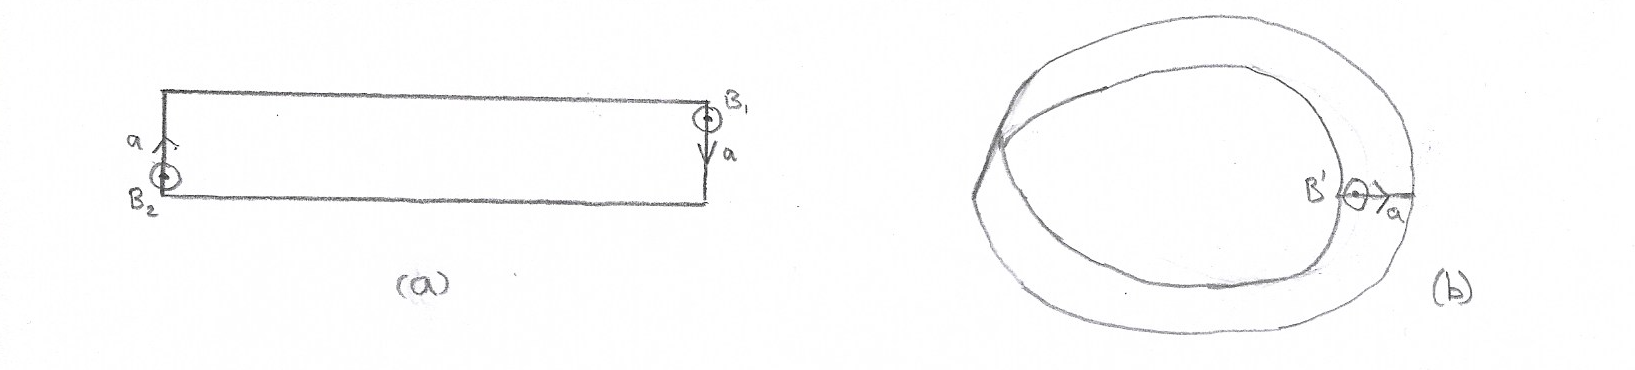
\includegraphics[width=13.5cm]{mobius.png}
  \caption{The M\"obius strip as a quotient topology formed by
    identifying opposite edges of a rectangle.} 
  \label{fig:mobius}
\end{figure}
\end{exmp}

This example is notable because it shows that surfaces can be
equivalently written as themselves that are  ``cut-up'' albeit
remembering which edges of the cut-up surface are ``to be
identified''. This information of which edges are to be identified is
conveyed by writing the cut-up surface as a quotient topology. We will
use this technique extensively in the next section (and throughout the
rest of this document) as we show that an arbitrary surface can be
``cut-up'' into triangles that are ``to be identified''.

\subsection{Triangulation}
\label{sec:surf:triangulation}

We define what it means to triangulate a surface.

\begin{defn}
  Given a surface $S$, we say that the collection of closed sets $\{
  T_1,  T_2, \dots T_n \}$ \emph{triangulates} $S$ if it covers $S$
  and for each $i = 1,2, \dots, n$ there exists homeomorphisms $\phi
  : T_i' \rightarrow T_i$ where each $T_i'$ is a triangle in
  $\mathbb{R}^2$ under the metric topology (described in example
  \ref{exmp:metric}). We say that the \emph{edges} of $T_i$ are images
  of the edges of $T_i'$ for each $i$; similarly the \emph{vertices}
  of $T_i$ are the images of the vertices of $T_i'$.
\end{defn}

We take it as a fact that any compact surface can be triangulated. We
understand that this is the case from the Jordan Curve theorem but
showing this goes beyond the scope of this project. To see a proper
discussion of how arbitrary compact surfaces can be triangulated,
refer to \cite{thom}.

Given that an arbitrary surface $S$ can be triangulated, we make
``cuts'' along the edges of the triangles and notice that each
triangle can be ``pasted'' onto the plane $\mathbb{R}^2$. Since
translations are homeomorphisms as well, we can translate the
triangles appropriately and have all triangles from the triangulation
``pasted'' on the plane in a manner by which they do not intersect
each other.

More formally, we begin by inductively relabeling our
triangulation. Suppose we have $n$ ``triangles'' that cover $S$; then
we proceed to label them inductively starting by labeling any
triangle $T_1$. Then, for each $1 \leq i \leq n-1$, choose a $T_{i+1}$
that has an edge $e_i$ in common with one of the preceding
triangles $T_1, T_2, \dots, T_i$. Such a triangle must always exist by
our implicit assumption of the connectedness of $S$. Numbering  our
triangle in this manner, we have defined the edges $e_i$ for $2 \leq i
\leq n$. 

For each triangle $T_i$ we must by definition have a homeomorphism
$\psi_i: T_i' \rightarrow T_i$, where $T_i'$ is a triangle in
$\mathbb{R}^2$. Translating the triangles $T_i'$ to $T_i''$ such that
they are pairwise disjoint, it is clear that there exists
homeomorphisms $\phi_i: T_i'' \rightarrow T_i$. Finally, given $T'' =
\cup_{i=1}^n T_i''$ and $\phi : T'' \rightarrow S$ defined via $\phi
\restriction T_i = \phi_i$ it is easy to see that $\phi : T''
\rightarrow S$ is a homeomorphism. 

For now, we assume that our surface $S$ doesn't have a
boundary and as a result each triangle edge has a corresponding edge %% what is a boundary?
on some other triangle that it is identified with.

Here we have explained how an arbitrary compact surface can be written
as finitely many triangles pasted on the plane \emph{under the
  quotient topology} that identifies pairs of edges. It is important
to note that we must include the added information of which edges are
identified with each other when we represent this quotient space, and
also include in what direction they are to be glued on. In 
particular we will represent this quotient space as the triangle that
forms it with each edge labeled and an it's identification
``direction''. We have already seen in Figure \ref{fig:mobius} how we
may imagine this space, where each edge is labeled with an arrow
indicating which direction it is to be identified with it's
corresponding edge.

We will show that the triangles of this quotient space can be
``glued'' onto one another so that we end up with a quotient space on
a geometric shape that is topologically equivalent to a disc. We do
this as follows.

It is clear that each $T_i$ is homeomorphic to a closed
disc. Furthermore, we have that the edges of $T_i$ are homeomorphic to
``closed'' boundaries on the disc, i.e.\ a set $A$ on the boundary of 
the disc that is homeomorphic to $[0,1]$. Now identifying two such
closed boundaries $A_1$ and $A_2$ we can identify them via the
homeomorphism between them and the resulting quotient space is
homeomorphic to a disc !(discuss). Hence, starting by deforming $T_1$
into a disc $D_1$, we proceed by gluing $T_i$ onto the edge $e_i$ of
the disc $D_{i-1}$ and continuously deform the resulting quotient
space into a disc $D_i$ for $2 \leq i \leq n$. Composing each gluing
and deformation, we have a surjective function $\pi$ from our quotient
space of triangles $T_1, T_2, \dots T_n$ to the disc $D_n$. Lemma
\ref{lem:prelims:compose} confirms that $\pi$ induces the quotient
topology on $D_n$ that is consistent with gluing each triangle and
deforming it into a disc one by one. As a result the boundary of the
disc entirely consists of the remaining pairs of edges i.e.\ not $e_2,
e_3, \dots, e_n$. Figure \ref{fig:square-pyramid} shows this process
being done for a square pyramid.

\begin{figure}[htbp]
  \centering
  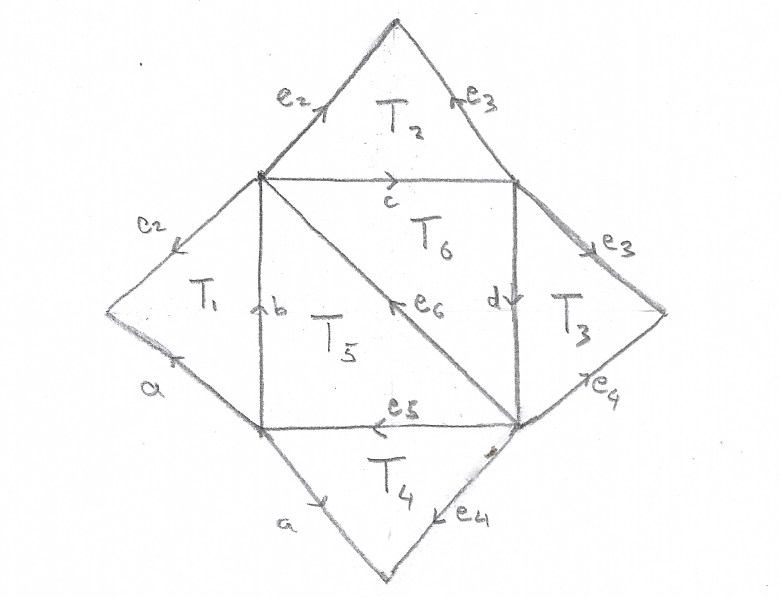
\includegraphics[width=8cm]{pyramid.png}
  \caption{Triangulating a square pyramid and forming its ``polygon''.}
  \label{fig:square-pyramid}
\end{figure}

This is significant since we formed a ``polygon'' that is homeomorphic
to an arbitrary compact and connected surface. Furthermore, if we
label the edges of the polygon, we can form a ``word'' that represents
the surface by going around the polygon counter-clockwise and picking
up the labels, with an inverse sign depending on the direction we
encounter them, and collating them. 

\subsection{Stating the Classification Theorem}
\label{sec:surf:thm}

Now that we know that a compact, connected surface $S$ can be written
as a polygon's quotient space all we seemingly need to do is classify
such polygons. Here we state the main theorem

\begin{thm}
  \label{thm:main}
  Any compact, connected surface without a boundary is either
  homeomorphic to a sphere, or to a connected sum of tori, or to a
  connected sum of projective planes. 
\end{thm}

We will now describe these ``prototype'' surfaces and show how they
can be written as polygons (and thus ``words'') as we did in section
\ref{sec:surf:triangulation}. Finally, we will show how an arbitrary
$D_n$ as formed in \ref{sec:surf:triangulation} can be reduced into
one of our ``prototype polygons''.


\subsubsection{The Sphere, Torus and Projective Plane}
\label{sec:surf:thm:stp}

Here we describe the prototype surfaces that are orientable, namely
the sphere and n-tori. The sphere is the simplest orientable surface
that we encounter. We can ``cut'' a slit along a diameter, pull the
sphere open and flatten it to form a bigon under the quotient topology
as demonstrated in figure \ref{fig:sphere-bigon}.

\begin{figure}[htbp]
  \centering
  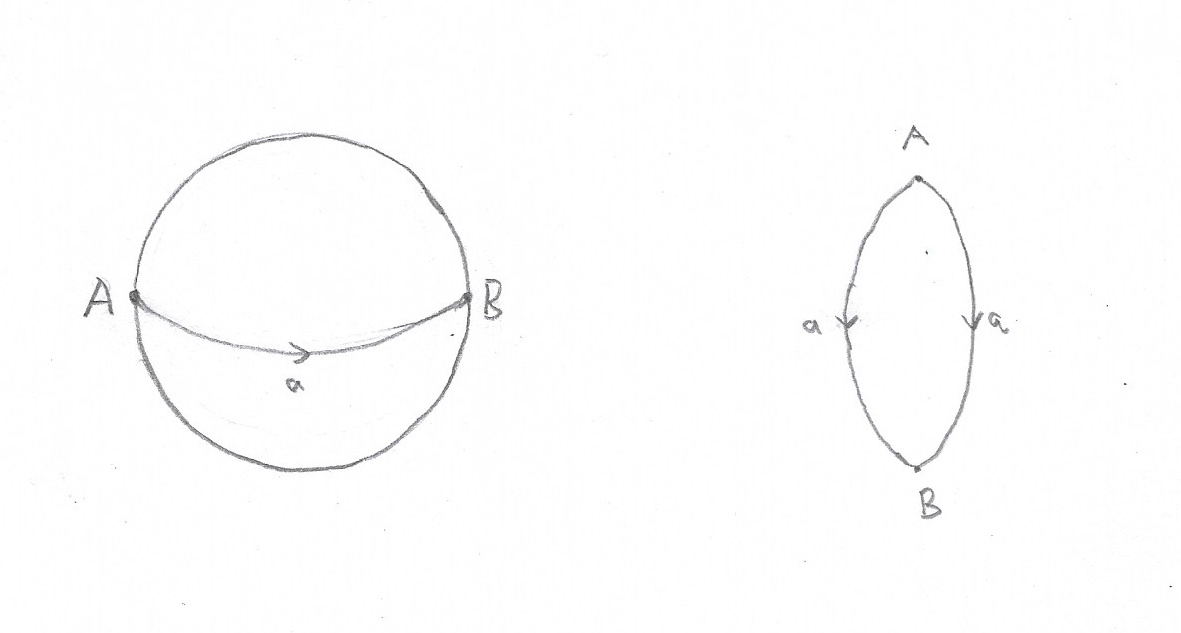
\includegraphics[width=14cm]{sphere.png}
  \caption{Representing the sphere as a bigon.}
  \label{fig:sphere-bigon}
\end{figure}

This polygon's quotient topology can be written, starting from the top
vertex and going counter-clockwise, as  the ``word''
$aa^{-1}$. Another simple surface that can be represented as a bigon,
albeit non-orientable is the projective plane; it is represented by
the quotient topology in figure
\ref{fig:projective-plane-bigon}. The corresponding word for this surface
is clearly of the form $aa$.

\begin{figure}[htbp]
  \centering
  
\includegraphics[width=13.5cm]{projective.png}
  \caption{The projective plane.}
  \label{fig:projective-plane-bigon}
\end{figure}

The last basic surface that we present in this section is the torus,
which is a simple tube whose edges are glued onto each other
(identified). This can be represented as a quadrilateral as in figure
\ref{fig:torus-rectangle}. The corresponding ``word'' takes the form
$aba^{-1}b^{-1}$ 

\begin{figure}[htbp]
  \centering
  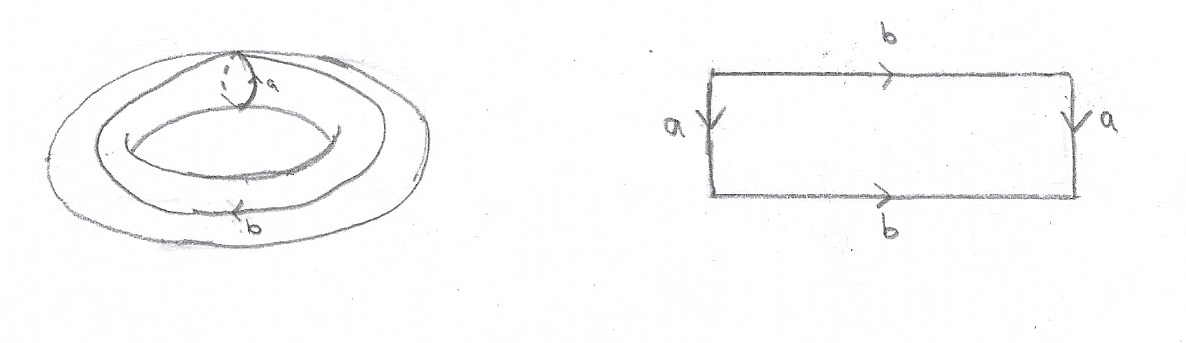
\includegraphics[width=8cm]{torus.png}
  \caption{Identifying edges of a rectangle to form a torus.}
  \label{fig:torus-rectangle}
\end{figure}

\subsubsection{Connected Sums}
\label{sec:surf:thm:cs}

For two disjoint surfaces, their connected sum is formed by deleting
circular holes in the surface and gluing the boundaries of the holes
to each other. More precisely we can do this to surfaces $S_1$ and
$S_2$ by taking two neighbourhoods $U_1 \subseteq S_1$ and $U_2
\subseteq S_2$ that are homeomorphic to the open unit disc via
$\phi_1$ and $\phi_2$. If $B_1$ and $B_2$ are open balls of radius
$\frac{1}{2}$ in the respective images of $\phi_1$ and $\phi_2$, we
form the connected sum $S$ by deleting the preimages of the interiors
of $C_1$ and $C_2$, i.e.\ we have $S_1' := S_1 \setminus
\phi_1^{-1}(B_1)$ and $S_2' := S_2 \setminus
\phi_2^{-1}(B_2)$. Finally we glue the boundaries of the deleted
balls, that is, we identify points in $\phi_1^{-1} (\partial B_1)
\subseteq S_1'$ with those in $\phi_2^{-1} (\partial B_2) \subseteq
S_2'$ to form our connected sum $S$ of $S_1$ and $S_2$. We know that
this can indeed be done since both are homeomorphic to circles in
$\mathbb{R}^2$.

First, we will study how connected sums of tori are formed. We already
know that tori can be written as quadrilaterals with opposite edges
identified; thus we can write  two tori $T_1$ and $T_2$ as
$a_1b_1a_1^{-1}b_1^{-1}$ and $a_2b_2a_2^{-1}b_2^{-1}$
respectively. Now cut out closed loops $c_1$ and $c_2$ in $T_1$ and
$T_2$ that run through the vertices  $a_1b_1^{-1}$ and $a_2b_2^{-1}$
respectively, as in figure \ref{fig:2-tori}. Now we identify the $c_1$
with $c_2$ to form the 2-torus represented by the polygon
$a_1b_1a_1^{-1}b_1^{-1}a_2b_2a_2^{-1}b_2^{-1}$.

\begin{figure}[htbp]
  \centering
  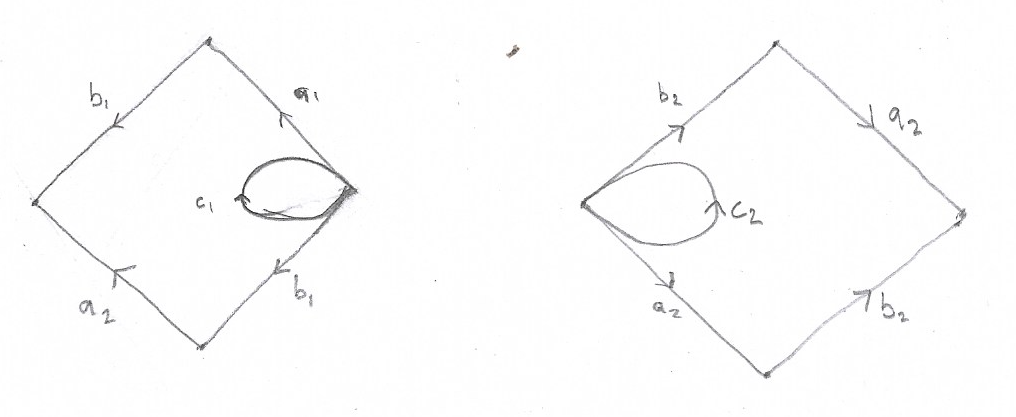
\includegraphics[width=12cm]{2torus.png}
  \caption{The 2-torus}
  \label{fig:2-tori}
\end{figure}

Cutting a loop that passes through the vertex between $a_1$ and
$b_2^{-1}$ we can connect another torus that we write as
$a_3b_3a_3^{-1}b_3^{-1}$ as we did above to form a $3-torus$ of the
form
$a_1b_1a_1^{-1}b_1^{-1}a_2b_2a_2^{-1}b_2^{-1}a_3b_3a_3^{-1}b_3^{-1}$. This
can be repeated $n$ times and thus an n-torus can be written as the
word $a_1b_1a_1^{-1}b_1^{-1}a_2b_2a_2^{-1}b_2^{-1} \dots
a_nb_na_n^{-1}b_n^{-1}$.

This process can be done to the projective plane as well by cutting
holes and gluing as in figure \ref{fig:2-projective-plane}. The word
we arrive at after one iteration is $a_1a_1a_2a_2$, but it is easy to
see that the connected sum of $n$ projective planes can be written as
the word $a_1a_1a_2a_2 \dots a_na_n$.

\begin{figure}[htbp]
  \centering
  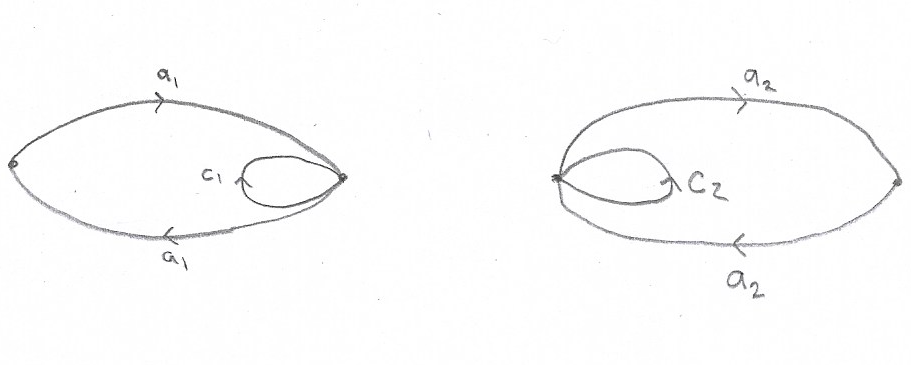
\includegraphics[width=12cm]{2projective.png}
  \caption{Connected sums of projective planes}
  \label{fig:2-projective-plane}
\end{figure}

With this we have introduced all of our prototype surfaces and  we
will proceed to present a lemma that will prove useful in proving the
classification theorem. 

\begin{lem}
  \label{lem:connected}
  The connected sum of a torus and a projective plane is homeomorphic
  to the connected sum of three projective planes. 
\end{lem}

Before we prove this lemma, it will be helpful to take a look at the
following example.

\begin{exmp}
  \label{exmp:klein} A Klein bottle is a non-orientable surface formed by identifying
  edges of a rectangle as in figure \ref{fig:klein}. We will see that
  this surface is equivalent to the connected sum of two projective
  planes.
  \begin{figure}[htbp]
    \centering
    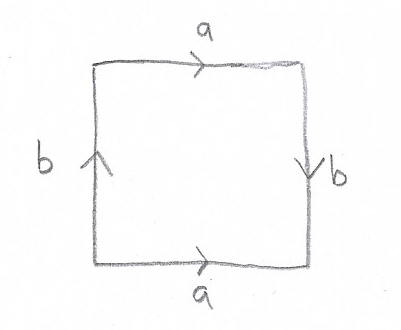
\includegraphics[width=8cm]{klein.png}
    \caption{The Klein Bottle}
    \label{fig:klein}
  \end{figure}
  Cutting out a disc $D_1$ from a projective plane $S_1$, we
  observe that the surface $S_1 \setminus D_1$ is a M\"obius strip as
  can be seen in figure \ref{fig:mob-proj}.
  \begin{figure}[htbp]
    \centering
    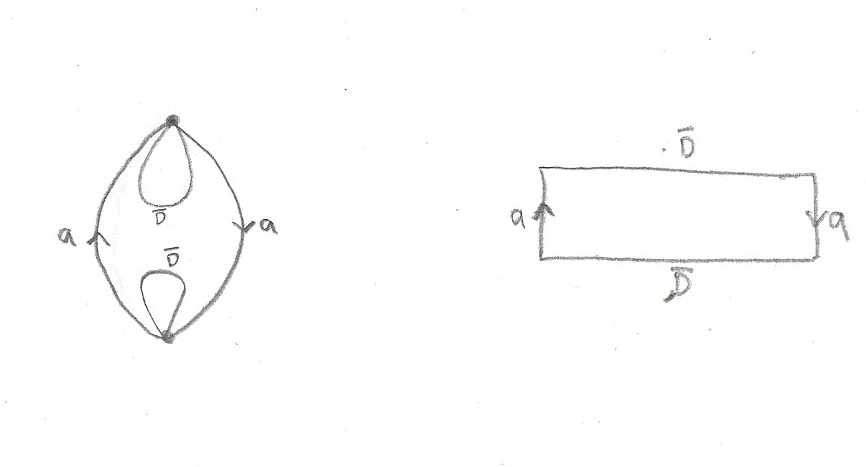
\includegraphics[width=13.5cm]{mobdisk.png}
    \caption{The M\"obius strip is a projective plane with a disc deleted}
    \label{fig:mob-proj}
  \end{figure}
  Thus, the connected sum of two projective planes $S_1$ and $S_2$
  must be two M\"obius strips glued onto one another at the
  boundary. From  figure \ref{fig:klein}, it is easy to see that this
  is indeed a Klein bottle.
\end{exmp}

\begin{proof}
  By example \ref{exmp:klein}, our problem is reduced to showing that
  the connected sum of the projective plane and Klein bottle is
  homeomorphic to the connected sum of the projective plane and
  torus. The canonical quotient spaces representation for the Klein
  bottle and torus with discs deleted are shown in figure
  \ref{fig:tor-klein}.
  \begin{figure}[htbp]
    \centering
    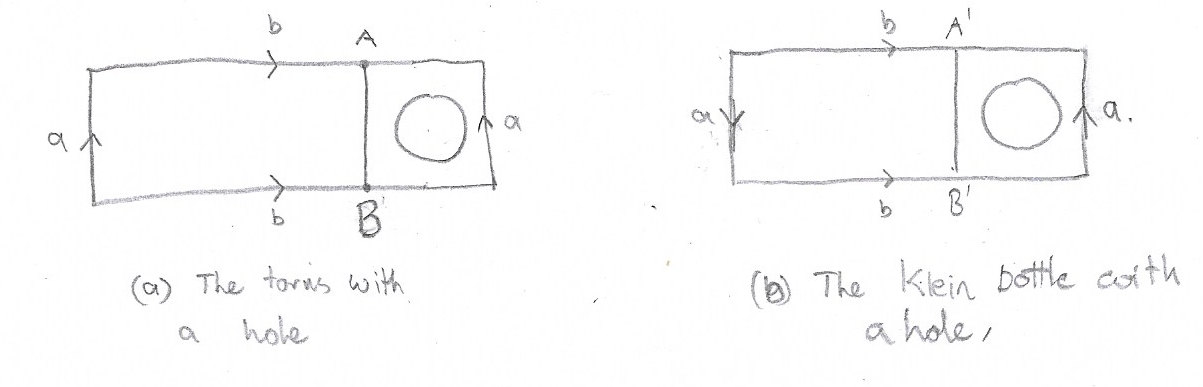
\includegraphics[width=13.5cm]{torklein.png}
    \caption{The torus and Klein bottle}
    \label{fig:tor-klein}
  \end{figure}

  We make cuts along $AB$ and $A'B'$, to form the edge $a'$. Gluing
  the hole in these cutoffs onto a hole in a segment of a surface is
  represented in figure \ref{fig:glue-S}. We have our surface with two
  holes to which the remainder of the Klein bottle or torus must be
  identified.

  \begin{figure}[htbp]
    \centering
    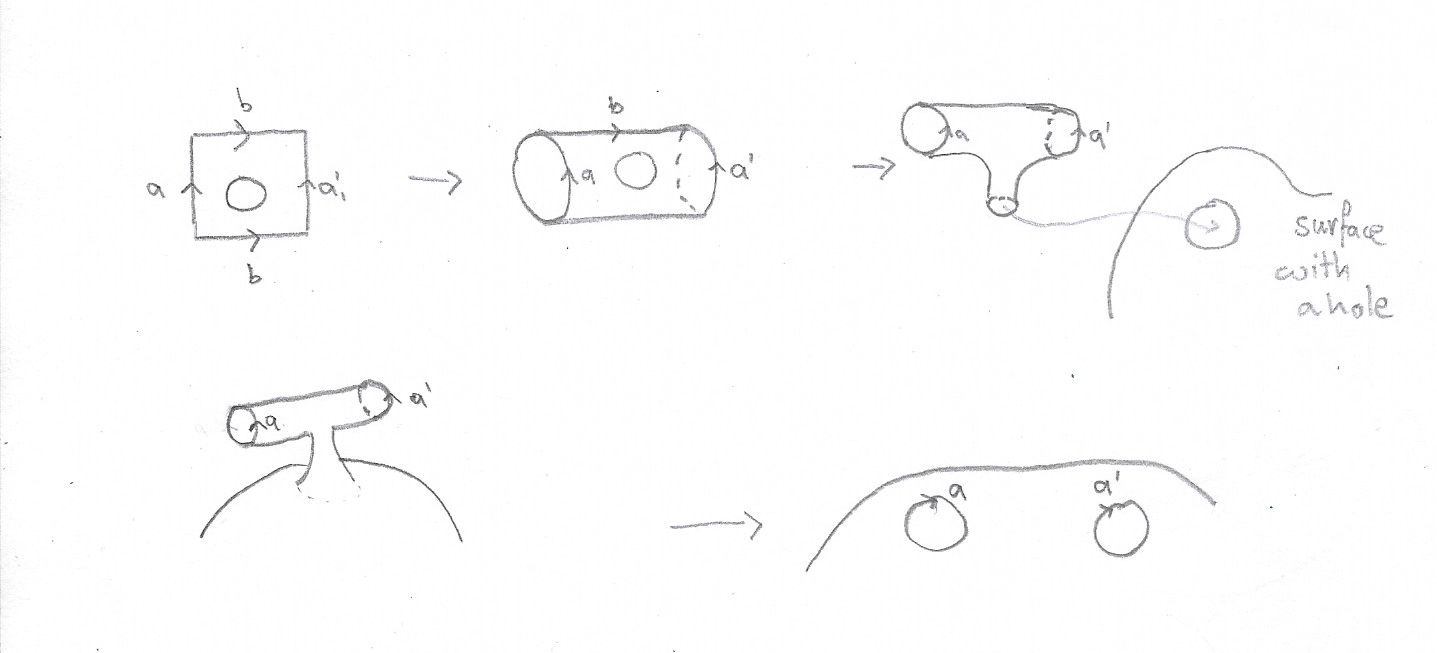
\includegraphics[width=13.5cm]{glues.png}
    \caption{The first step of gluing the torus and Klein bottle onto
      a surface segment}
    \label{fig:glue-S}
  \end{figure}

  In our second stage of gluing we want to re-attach the segment we cut
  away in figure \ref{fig:tor-klein}. Here we will suppose that the
  surface we are gluing to is a M\"obius strip. The completion of the
  second stage in both the case of the torus and the Klein bottle is
  seen in figure \ref{fig:glue-mob}, working in the M\"obius strip as a
  quotient topology that is cut apart at $m$.
  
  \begin{figure}[htbp]
    \centering
    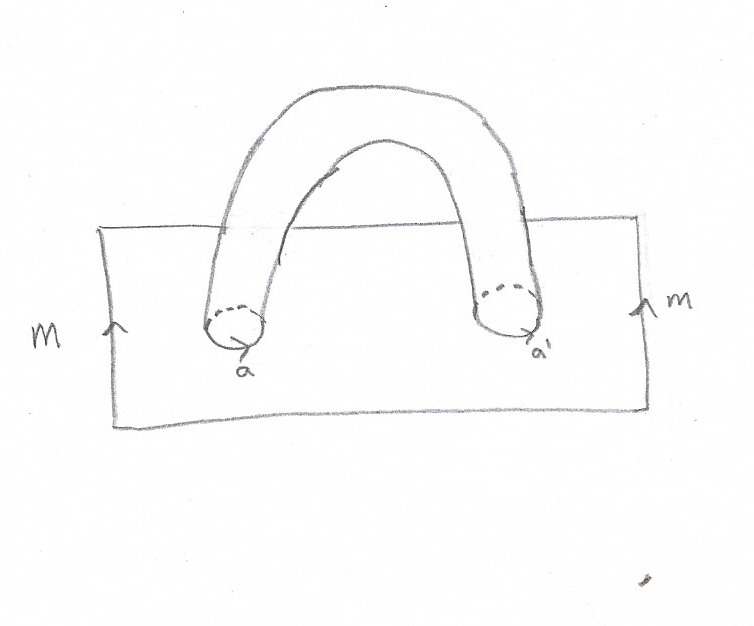
\includegraphics[width=8cm]{gluemob.png}
    \caption{The connected sums of the torus and the Klein bottle with
      the M\"obius strip}
    \label{fig:glue-mob}
  \end{figure}
  Since the M\"obius strip is simply a projective plane with a disc cut
  out as seen in example \ref{exmp:klein}, we just could have
  identified the boundary of a disc with the boundary of the M\"obius
  strip and have our result.
\end{proof}

In summary the canonical forms given in theorem \ref{thm:main} can be
written as follows. 

\begin{itemize}
\item The sphere, written as $aa^{-1}$.
\item The connected sum of $n$ tori,  written as
  $a_1b_1a_1^{-1}b_1^{-1}a_2b_2a_2^{-1}b_2^{-1} \dots
  a_nb_na_n^{-1}b_n^{-1}$.
\item The connected sum of $n$ projective planes, written as
  $a_1a_1a_2a_2 \dots a_na_n$.
\end{itemize}

 \begin{proof}[Proof of the Classification Theorem]
   This now simply boils down to showing that the polygon $D_n$ that
   we constructed from an arbitrary surface in section
   \ref{sec:surf:triangulation} is homeomorphic to one of the three
   above forms. We do this by manipulating $D_n$ in a systematic way
   to arrive at one of these forms.

   First, we will classify the pairs of edges of $D_n$. We say that
   pairs that occur in opposite directions are \emph{pairs of the
     first kind}; an edge with the label $a$ will occur as a pair of
   the first kind in $D_n$ if $D_n$'s word has the exponents of the
   two occurrences of the label $a$ not equal. In other words, $a$ and
   $a^{-1}$ both appear in the word representing $D_n$. For example a
   sphere is nothing but a pair of the first kind. On the other hand
   we call \emph{pairs of the second kind} those pairs who both have
   the same exponents. For example a projective plane is simply a
   single pair of the second kind.

   We can eliminate adjacent pairs of the first kind in any polygon
   with more than two pairs by simply identifying the pair as seen in
   \ref{fig:first-adjacent}. Thus $D_n$ can be reduced to a polygon
   with no adjacent pairs of the second kind or a bigon, which we know
   is equivalent to either a sphere or a projective plane. In the
   latter case we are done so assume that $D_n$ is reduced to $P$, a
   polygon with no adjacent edges of the first kind. Figure
   \ref{fig:square-pyramid} is found to be homeomorphic to the sphere
   by this step.

   \begin{figure}[htbp]
     \centering
     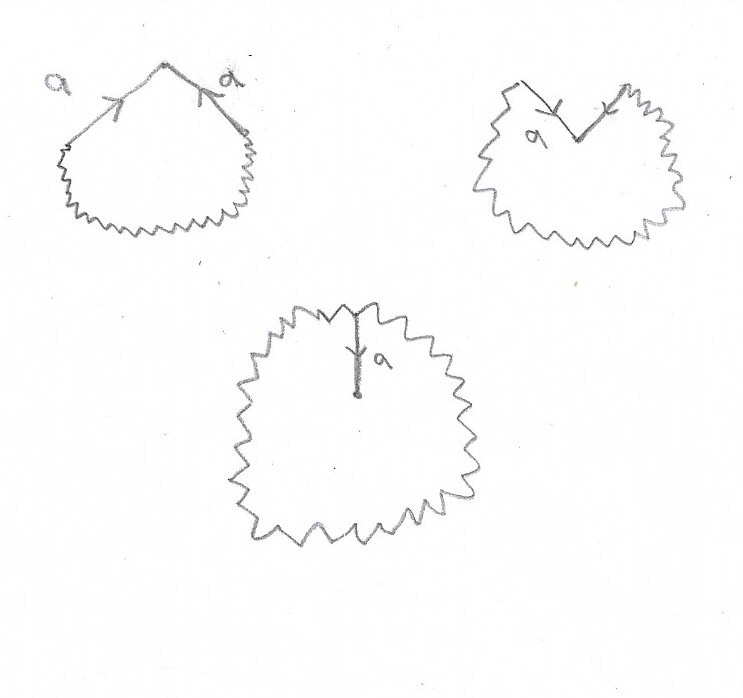
\includegraphics[width=8cm]{first.png}
     \caption{Eliminating adjacent pairs of the first kind.}
     \label{fig:first-adjacent}
   \end{figure}

    Just as edges were formed by cutting and are to be reidentified, so
    are vertices; however, unlike edges, vertices need not be identified
    in pairs. Rather, an equivalence class of vertices may have any
    finite number of vertices along the polygon $P$. 
    
    We claim that all but one equivalence class of vertices can be
    eliminated via homeomorphic actions on the polygon $P$. Suppose
    there are at least two equivalence classes of vertices. In this
    case, we will show that an arbitrary equivalence class $A$ can be
    eliminated. This will clearly lead to our claim being verified
    since we have finitely many equivalence classes of vertices.

    $A$ must have a vertex that is adjacent to a vertex of a different
    equivalence class, say $B$. Since we have eliminated adjacent
    pairs of edges the first kind, an equivalence class of vertices
    such as $A$ must have more than one vertex, therefore without loss
    of generality we can represent our situation as in figure
    \ref{fig:vertex-eliminate} (a). With this figure in mind, 
    cut the polygon along $c$ and identify the pair of edges $a$, as
    pictured in part (b) of the figure. We now have one fewer vertex
    of the equivalence class $A$ and one more of the equivalence class
    $B$. Now, apply the first step again (eliminate adjacent pairs of
    the first kind). Either this will eliminate the class $A$ if a
    single vertex remains, or we will have the conditions required to
    repeat this procedure till finally $A$ is eliminated.
    
    \begin{figure}[htbp]
     \centering
     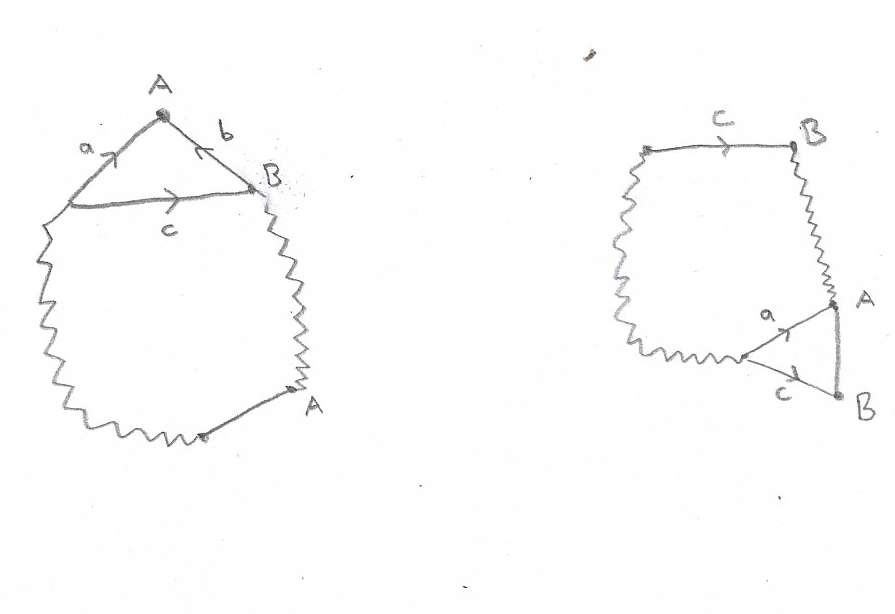
\includegraphics[width=10cm]{vertex.png}
     \caption{Reducing the number of vertices in an equivalence class
       of more than one vertex.}
     \label{fig:vertex-eliminate}
   \end{figure}

   Now we can make a pair of the second kind adjacent by the procedure
   pictured in figure \ref{fig:second-adjacent}. Note that this neither
   separates adjacent pairs, nor does it create a new equivalent class
   of vertices. Thus, this can be done finitely many times to make all
   pairs of the second kind adjacent.

   \begin{figure}[htbp]
     \centering
     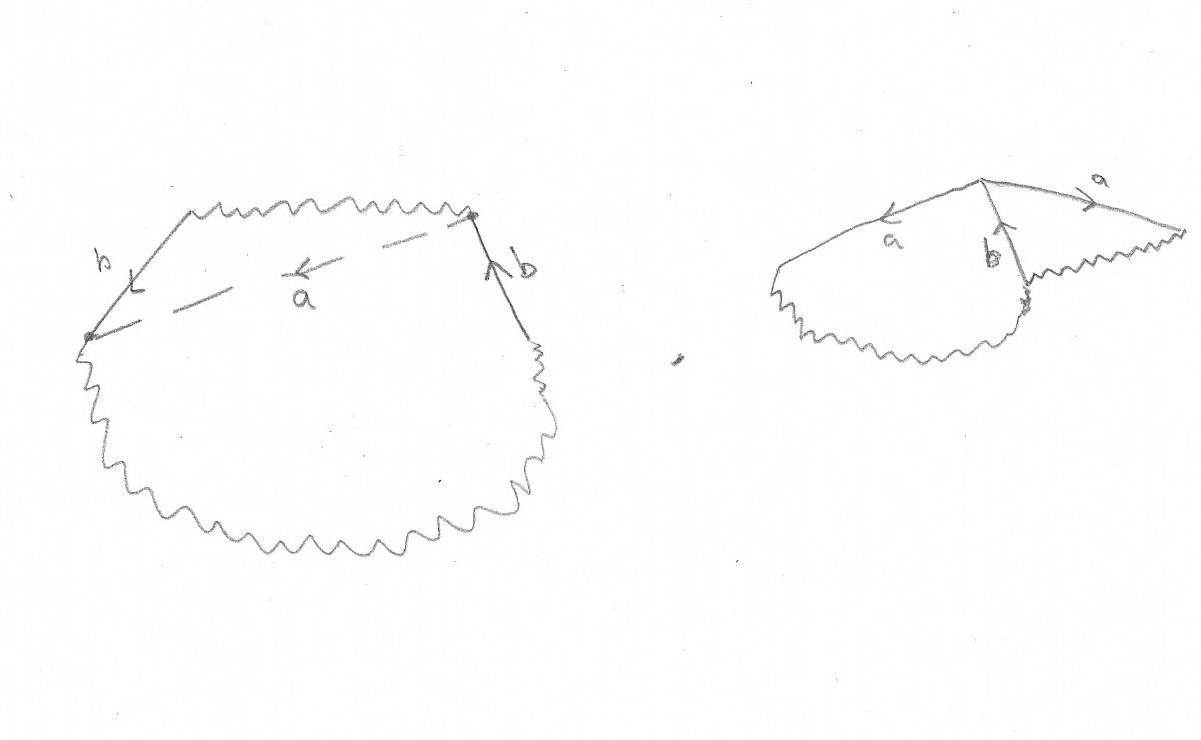
\includegraphics[width=10cm]{second.png}
     \caption{Making pairs of the second kind adjacent.}
     \label{fig:second-adjacent}
   \end{figure}

   If no pairs of the first kind are present at this stage, our
   polygon is of the form $a_1a_1a_2a_2 \dots a_na_n$: a connected sum
   of $n$ projective planes and we are done. We continue with the
   assumption that a pair of the first kind yet exists.

   We claim that a pair of the first kind must be separated by an edge
   of another pair of the first kind. To the
   contrary, consider the figure \ref{fig:first-contradiction}, where
   $A$ and $B$ respectively represent a sequences of pairs of the
   second kind (there are no pairs of the first kind other than $c$
   and $c^{-1}$ in the figure). Now by the step we have just
   completed, all pairs of the second kind are adjacent to one
   another. This means that each edge in $A$ has it's corresponding
   edge in $A$ and the same is true for $B$. But this means that
   the vertex at the origin and end of $c$ can't be identified with
   one another (the edges connecting to either end can never match),
   which means that we have at least 2 distinct equivalence classes of
   vertices, a contradiction of our previous step.

   \begin{figure}[htbp]
     \centering
     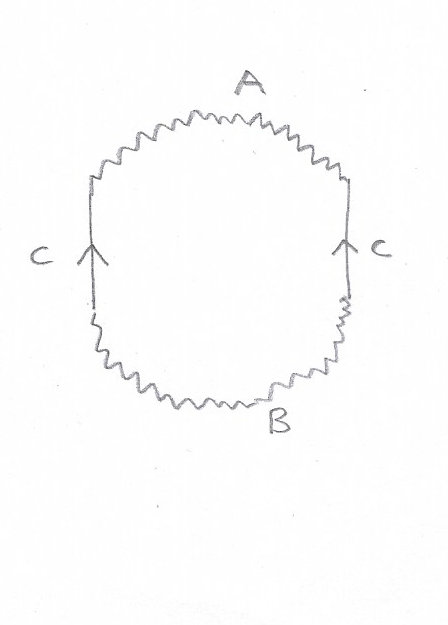
\includegraphics[width=8cm]{contr.png}
     \caption{A pair of the first kind separated on either side only
       by pairs of the second kind.}
     \label{fig:first-contradiction}
   \end{figure}

   Thus we assume that each pair of the first kind alternates with
   another pair of the first kind. The transformation pictured in
   figure \ref{fig:last} shows us how we can make these four edges
   adjacent. Now we can repeat this such that edges of the first kind
   always occur in fours. If no pairs of the second kind remain, we
   clearly have a connected sum of tori.

   On the other hand, if pairs of the second kind do remain, two
   alternating pairs of the second kind must be adjacent to such a
   pair. But lemma \ref{lem:connected} shows us that such an
   arrangement is equivalent to the connected sum of three projective
   planes; thus the whole polygon reduces to the connected sum of
   projective planes.

   \begin{figure}[htbp]
     \centering
     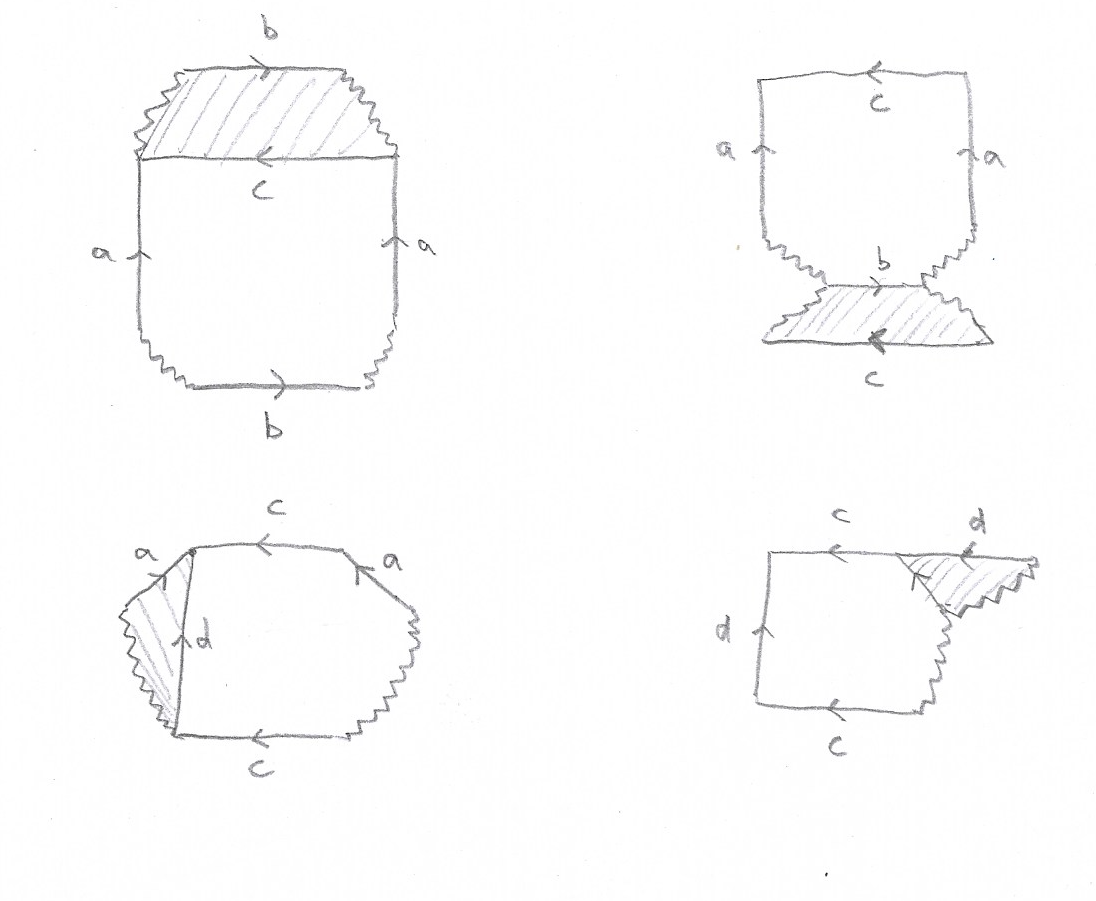
\includegraphics[width=8cm]{las.png}
     \caption{A pair of the first kind separated on either side only
       by pairs of the second kind.}
     \label{fig:last}          
   \end{figure}
 \end{proof}

 Thus we have classified an arbitrary compact connected surface without a boundary by triangulating it and forming a polygon from the triangulation which we manipulate into a canonical form. Our theorem can be extended without much difficulty to show that the compact surfaces with boundaries can be similarly classified into spheres or connected sums of projective planes and tori, however for each boundary present, we cut out a disc from the canonical surface. We have already seen this in the case of the M\"obius strip which is simply a projective plane with a disc cut out.



%%% Local Variables:
%%% mode: latex
%%% TeX-master: "main"
%%% End:



\end{document}

%%% Local Variables:
%%% mode: latex
%%% TeX-master: t
%%% End:
